\section{Simulation of users behaviors}
On past semester the Security Group of the chair "Internet Technologies and Systems" worked on the project "Machine Learning for Security Analytics powered by SAP HANA". Within this project the group aim to implement and test the machine learning approach for security analytics based on SAP HANA. Under this approach the group focuses on the analysis of user events, particularly login and logout events. For testing of machine learning analytics module, we have generated several simple brute-force attacks. As a result the project report was written that contains the results of applying machine learning approach, analyzing of performance and other relevant information. [?!? link to the report]. Also it contains the proposals of future works. And one of them was a proposal to try machine learning approach powered on SAP HANA for security Analytics with more sophisticated cases. But the main problem of trying the approach on sophisticated cases is a lack of data. The lack of data is common problem of academic world. Mostly, only industrial companies has such data in needed amount but they do not share them because of some obviously reasons such as security and privacy. At least login and logout events contain information about users that can not be passed to third parties. For the reason we faced with task to implement a tool to simulate particular user scenarios, user behaviors and as result generate needed data for future analyzing. 
The Scenario in our case is a description of a network infrastructure, an information about users and a description of their behaviors. To analysis user behaviors by predict algorithms of machine learning approach we must have a normal scenario and an abnormal scenario.  
  
\subsection{Environment description}
We start with designing a network and a description of the network. It contains the list of computers, which operations systems are installed, purposes of each machine and list of users with their roles. The main node of the network is Domain controller (DC). On Domain controller the Widows Sever 2012 was used. Additionally we added two virtual machines with Windows Server 2013 that are used as Wiki server and Database server accordingly. Also the network contains 4 user virtual machines with Windows 7 64 bit Pro. To complete the installation we add 4 users and 1 of them is Admin user who has an access to any machines. All described information is summarized into two compacted list below. 

Description of a network:
\begin{compactitem}
\item 4 user computers with Windows 7 64-bit Pro.
\item Domain controller with Widows Server 2012.
\item Wiki server with Windows Server 2013.
\item Database (DB) server with Windows Server 2013.
\end{compactitem}
Users: 
\begin{compactitem}
\item Ivanov
\item Petrov
\item Smirnov
\item Admin
\end{compactitem}
     
\subsection{Normal scenario}
All users has an access to user computers, Wiki server and Database server. Admin has an access to any computer such as user computers, Wiki server, DB server, Domain Controller. In case of normal scenario ordinal users usually login to user computers by their credentials. They do it several times per day. Petrov and Smirnov during a workday go to Wiki server. Ivanov does not go there despite that he has an access. As was mentioned above all users have access to DB Serve, but nobody uses it. Admin usually login to his computer and during a workday he connects to Domain Controller, DB server and Wiki server several time. Is is clear that other user do not connect to Domain Controller because they do not have an access. The visualized description of normal behavior you can see on the Figure 1: Normal scenario. All black lines show  accesses to computers for particular users. The black solid lines illustrate accesses which are used by users. The black dash lines show accesses which are not used by users in the normal behavior despite that they have an access. 
\begin{figure}[ht!]
\centering
%[width=90mm]
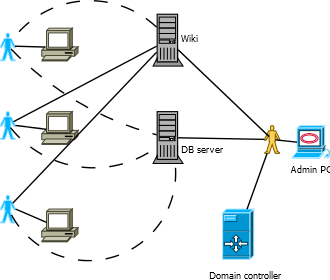
\includegraphics{scenario_normal.png}
\caption{Normal scenario}
\label{overflow}
\end{figure}

\subsection{Abnormal scenario}
The abnormal scenario is some kind of scenario that differs from normal scenario by some unusual but acceptable behaviors. In our case abnormal scenario includes additional user behaviors. The first abnormal behavior is that user Ivanov uses Wiki server. It is abnormal, but not so much suspicious, because other users use it every day. The second abnormal behavior is that user Petrov start to use DB server, but in the normal scenario nobody use it. This user  behavior is more suspicious and could be determine as an attempt to hack the system. The abnormal scenario is illustrated on the Figure 2: Abnormal scenario. The black solid lines show normal user behaviors. The yellow solid line shows the first abnormal behavior connection to Wiki server. The red solid line show the second abnormal behavior that is suspicious and could be determined as an attempt to hack the system. 
\begin{figure}[ht!]
\centering
%[width=90mm]
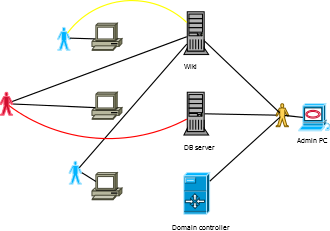
\includegraphics{scenario_abnormal.png}
\caption{Abnormal scenario}
\label{overflow}
\end{figure}

\subsection{Implementation}
The first part of the implementation is the deployment and configuration the test environment.  To set up the network we use FutureSOC server with installed WMware ESXi, because it has needed computer resources. Firstly, on the WMware ESXi network we create the VLAN network to isolate of virtual machines from others hosted on the same ESXi server. Then all machines was deployed and configured as described in the section "Environment description" [2.1]. We used Windows Server 2012 for Domain controller, Windows Server 2003 for Wiki server and DB server, Windows 7 64-bit Pro for user computers including admin's computer. 

The simulation of user behaviors is implemented by Python programming language with additional libraries. We call the python script for simulation of user behaviors "simulator". To connect from simulator to VMs the virtual Network Computing (VNC) protocol was used, because ESXi supports the VNC protocol. But it is needed to enable the VNC features on ESXi server and specified port for a vnc connection for each VM. To connect to VM by VNC we used vncdotool library ([!? link  https://github.com/sibson/vncdotool]). The library supports not only connecting to VMs by VNC, but also it can make screeshots of the VM desktop. The feature of making sreenshot of the VM desktop is used for checking a state of the VM. The simulator describe the algorithm of user behavior for connection to VM, login into OS, run RDP connection to Wiki or DB server. We predefined some common state to determine the current state of VM during the simulation by comprising histograms of images. By comparison images and determine the current state of VM we can specify activities that are needed to perform in any particular case according to a description of scenario. For example, if after comparison we determined that the state is "Logoff state" then we need pass CTL+ALT+DELETE command to VM to enable "Logon" state. In turn, in "Logon" state we can type an username and a password and press enter to enter to into the VM. The connection from the user computer to DB or Wiki server is implemented by running PowerShell Script hosted in VM. The script could take parameters and it means that we use one script for connection to both servers by specifying the certain IP address. The script establishes the RDP connection. 

In two above paragraph we described how we deploy, configure and connect to server. In this paragraph we describe how we describe the scenario of user behaviors. The description of scenarios is stored in csv files. The are 3 csv files. The first of them (computers.csv) describe the all computers which participate in the scenario. It contains the information about computer identifier (Id), IP address or host, port specified for VNC connection, VNC password and type of operation system (OS).
The second files is called scenarios.csv. It describes the main user activities. The main user activity means the connection to the user computer. The file contains a computer ID referring to id in computer.csv file, an username, a password, a session time, a count of sessions and identifier of inner scenario. The third files is called inner-scenarios.csv. It describes the user activity after login into a user computer. For example, it could describe the connection to the Wiki, the DB server or Domain controller or even connection to another user computer. The files contains Id, host, username, password, session time. There are two sets of csv files. The first set is used to perform the normal scenario and the second is used to perform the abnormal scenario accordingly. The described relations between csv files and content of csv files are illustrated on the Figure 3: Scenario relations.
 	
\begin{figure}[ht!]
\centering
%[width=90mm]
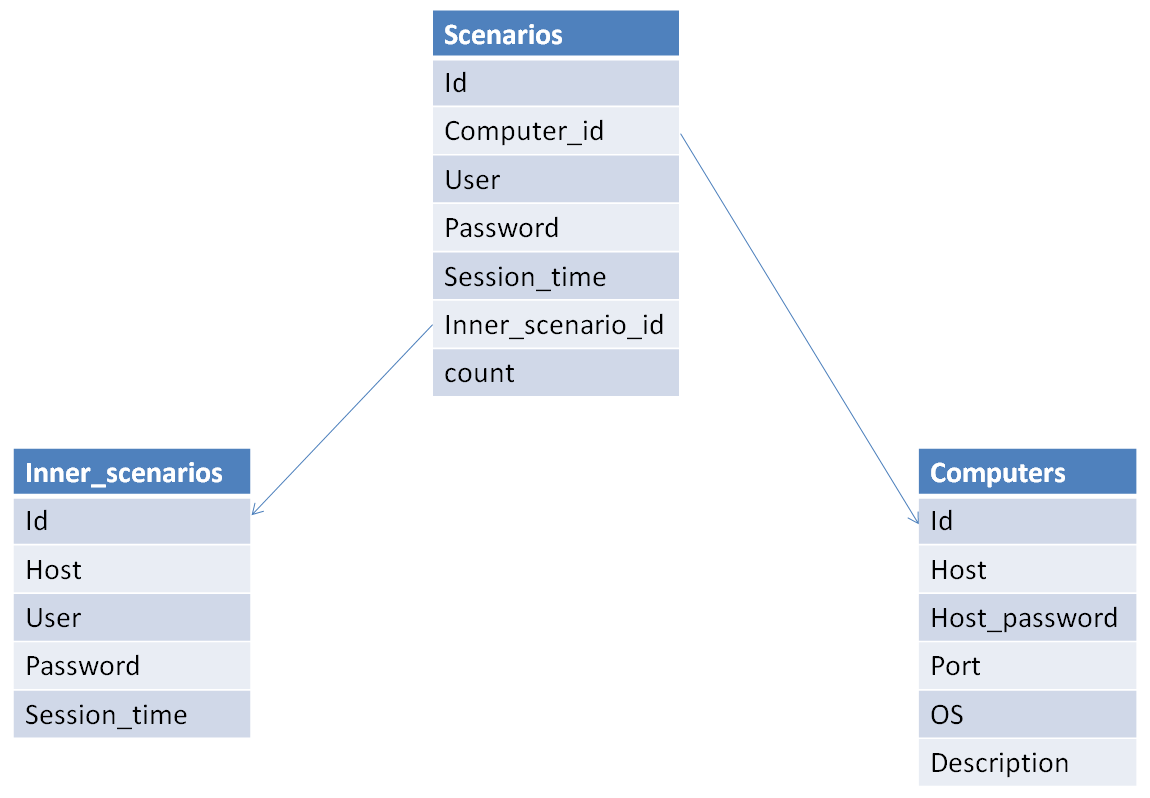
\includegraphics[width=150mm]{scenario_relations.png}
\caption{Scenario relations}
\label{overflow}
\end{figure}


The normal scenario takes about 3,5 hours with 41 login and logout events to user computers and 25 to Wiki and DB servers. The abnormal scenario takes about 5,5 hours with 45 login and logout events to user computers and 34 to Wiki and DB servers.
 
%\end{document} 